%!TEX TS-program = xelatex
\documentclass{EdipyLabs} % Custom class provided for EDIPY labs, by Christos Dalamagkas (cdalamagkas@gmail.com)
\SetLabNumber{2β}
\SetLabTitle{Διευθέτηση μεταγωγέα}
\SetAuthor{Χρήστος Δαλαμάγκας}
\SetLabDescription{Βασική παραμετροποίηση μεταγωγέων, ο πίνακας MAC, στατικές/δυναμικές διευθύνσεις MAC, ασφάλεια θυρών.}
\SetLabPrerequisites{Εργαστηριακό φυλλάδιο 1α (Εισαγωγή στο Cisco IOS), Βασική ορολογία δικτύων υπολογιστών, ειδικότερα όσον αφορά το επίπεδο ζεύξης δεδομένων.}

\begin{document}

\Initialize

\section*{Εισαγωγή}
Αντικείμενο του παρόντος εργαστηριακού φυλλαδίου αποτελεί η επισκόπηση της λειτουργίας των μεταγωγέων, καθώς και η επισκόπηση βασικών εντολών χειρισμού τους. Στο πλαίσιο της εργαστηριακής άσκησης θα υλοποιήσετε την τοπολογία που φαίνεται στο σχήμα \ref{fig:topology-generic}, η οποία αποτελείται από έναν μεταγωγέα, δυο υπολογιστές και έναν δρομολογητή. Η εργαστηριακή άσκηση αποτελείται από ένα σενάριο, το οποίο δίνει έμφαση στις κολλώδεις διευθύνσεις MAC.

\begin{figure}[H]
	\centering
	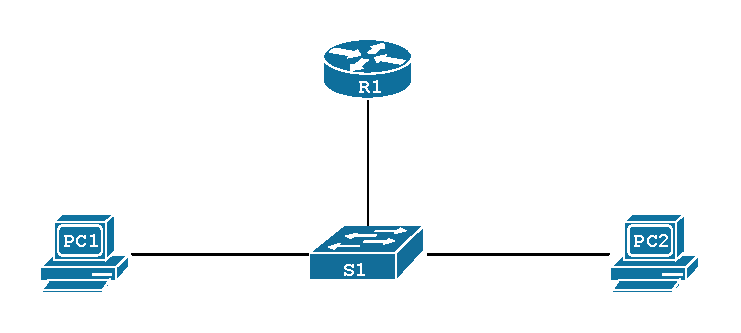
\includegraphics[width=\linewidth]{topology-generic}
	\caption{Βασικό σχέδιο της δικτυακής τοπολογίας}\label{fig:topology-generic}
\end{figure}

Για την υλοποίηση της τοπολογίας θα χρειαστείτε τις εξής συσκευές:
\begin{itemize}
	\item x1 δρομολογητή Cisco 2921
	\item x2 μεταγωγείς Cisco Catalyst
	\item x2 υπολογιστές
\end{itemize}


\section{Θεωρητικό υπόβαθρο}
Ο μεταγωγέας (switch) είναι μια συσκευή που λειτουργεί κατά βάση στο δεύτερο στρώμα του OSI (στρώμα ζεύξης δεδομένων - data link layer) και χρησιμεύει για την προώθηση πλαισίων στο εύρος ενός δικτύου. Ουσιαστικός ρόλος ενός μεταγωγέα είναι να επιτρέπει την πολλαπλή πρόσβαση συσκευών στο ίδιο φυσικό μέσο μετάδοσης. Για παράδειγμα, στο σχήμα \ref{fig:topology-generic} η χρήση του μεταγωγέα επιτρέπει και στους δυο υπολογιστές να έχουν πρόσβαση στο ίδιο φυσικό μέσο, δηλαδή τη ζεύξη με τη διεπαφή του R1.

Στα παρακάτω σημεία συνοψίζονται οι βασικές ιδιότητες των μεταγωγέων που τους διαχωρίζει από τους δρομολογητές:
\begin{itemize}
	\item Σε αντίθεση με τον δρομολογητή, ο οποίος προωθεί πακέτα μεταξύ διαφορετικών δικτύων, οι μεταγωγείς προωθούν πλαίσια μόνο μέσα στο εύρος του φυσικού δικτύου στο οποίο ανήκουν (τομέας ευρυεκπομπής - broadcast domain).
	\item Ο δρομολογητής επικοινωνεί με διαφορετικά δίκτυα με χρήση διεπαφών (interfaces), ενώ ο μεταγωγέας επικοινωνεί με το δίκτυο χρησιμοποιώντας θύρες (ports). Ουσιασικά, οι θύρες των μεταγωγέων είναι γεφυρωμένες διεπαφές (bridged interfaces), δηλαδή έχουν κατασκευαστεί ώστε να ανήκουν στον ίδιο τομέα ευρυεκπομπής.
	\item Οι δρομολογητές λαμβάνουν αποφάσεις προώθησης πακέτων εξετάζοντας τον πίνακα δρομολόγησης. Αντίθετα, οι μεταγωγείς λαμβάνουν απόφαση για το που θα προωθήσουν ένα πλαίσιο, εξετάζοντας τον πίνακα MAC.
	\item Οι δρομολογητές είναι ΚΑΙ μεταγωγείς, με τη διαφορά ότι κάθε διεπαφή ενός δρομολογητή βρίσκεται σε διαφορετικό φυσικό μέσο (τομέα ευρυεκπομπής) από τις υπόλοιπες. Συνεπώς, ο δρομολογητής επικοινωνεί σε επίπεδο μεταγωγής μόνο με τη συσκευή με την οποία συνδέεται απευθείας.
	\item Οι περισσότεροι μεταγωγείς ενεργοποιούνται αυτόματα, όταν συνδεθούν στην τροφοδοσία ρεύματος. Αντίθετα, οι δρομολογητές διαθέτουν διακόπτη τροφοδοσίας. 
	\item Σε αντίθεση με τις διεπαφές του δρομολογητή, οι θύρες των μεταγωγέων δεν χρειάζονται καμία ρύθμιση για να καταστούν λειτουργικές. Σε περίπτωση που συνδεθεί σε μια θύρα καλώδιο βύσματος RJ-45, και το έτερο άκρο δίνει ήδη τάση, τότε η θύρα ενεργοποιείται αυτόματα και είναι έτοιμη να προωθήσει πλαίσια. 
\end{itemize} 
  \newpage
  
\section{Υλοποίηση τοπολογίας}

\subsection{Αναλυτική σχεδίαση τοπολογίας}
Όπως και στο προηγούμενο μέρος του εργαστηριακού φυλλαδίου, πριν την υλοποίηση της τοπολογίας θα πρέπει πρώτα να καθοριστεί η αναλυτική τοπολογία του δικτύου, δηλαδή να προσδιοριστούν τα δίκτυα (ή το δίκτυο) που συνθέτουν την τοπολογία, οι διευθύνσεις IP και οι διεπαφές που θα χρησιμοποιηθούν. Η αναλυτική σχεδίαση της τοπολογίας φαίνεται στο σχήμα \ref{fig:topology-1} και το αντίστοιχο σχήμα διευθυνσιοδότησης στον πίνακα \ref{tab:addr}.

\begin{figure}[H]
	\centering
	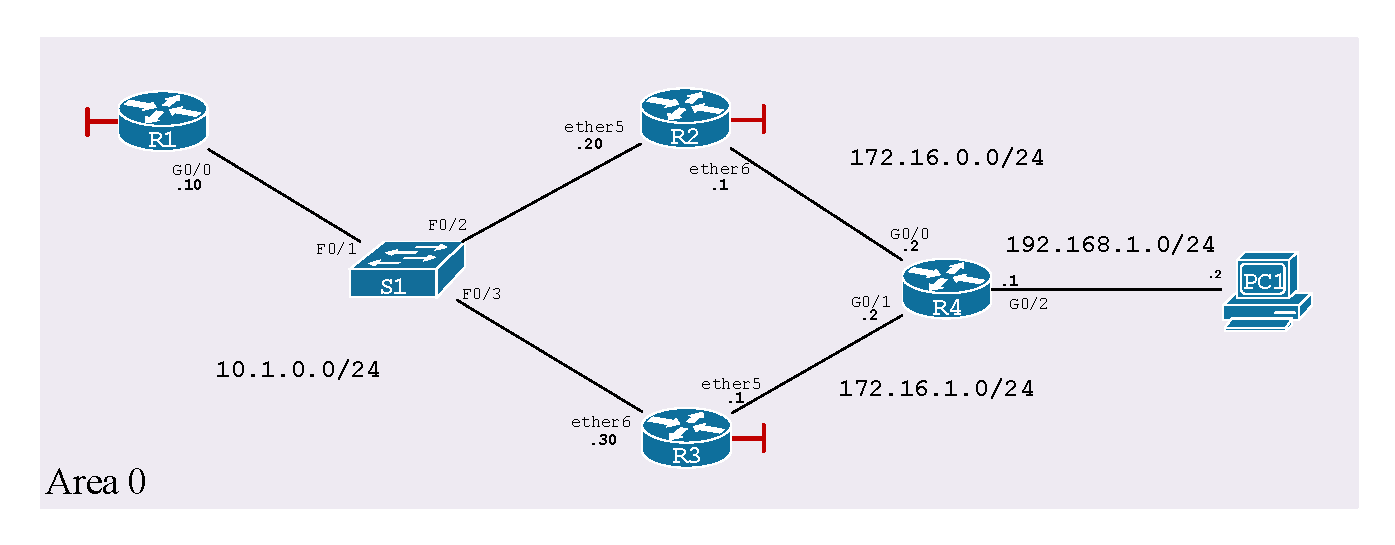
\includegraphics[width=\linewidth]{topology-1}
	\caption{To σχέδιο της αναλυτικής τοπολογίας προς υλοποίηση.}\label{fig:topology-1}
\end{figure}

\begin{IpAddressTable}{Σχήμα διευθυνσιοδότησης της τοπολογίας}{addr}
	R1				 & \ip{G0/0}		& \ip{192.168.1.1}	 	& \ip{255.255.255.128} & - \\
\rowcolor{lightgray}
	S1				 & \SVI				& \ip{192.168.1.127}	 	& \ip{255.255.255.128} & \ip{192.168.1.1}\\
	PC1 			 & \NIC	  			& \ip{192.168.1.10}	 	& \ip{255.255.255.128} & \ip{192.168.1.1} \\
\rowcolor{lightgray}
	PC2				 & \NIC	  			& \ip{192.168.1.20}	 	& \ip{255.255.255.128} & \ip{192.168.1.1}
\end{IpAddressTable}

\subsection{Καλωδίωση δικτύου}
Ως αρχικό βήμα, συνδέστε με καλώδια UTP τις συσκευές μεταξύ τους, όπως φαίνεται στο σχήμα της τοπολογίας. Αν δεν είναι δυνατό να χρησιμοποιήστε τις διεπαφές που φαίνονται στο σχήμα τοπολογίας, τότε αποφασίστε εσείς για τις διεπαφές που θα χρησιμοποιήσετε.

\subsection{Παραμετροποίηση μεταγωγέα}

Συνδεθείτε με κονσόλα στις συσκευές Cisco, σύμφωνα με τις οδηγίες του φυλλαδίου «Εισαγωγή στο Cisco IOS», και βεβαιωθείτε ότι αυτές λειτουργούν με τις εργοστασιακές τους ρυθμίσεις. Αν εντοπίσετε παλαιότερες ρυθμίσεις, επαναφέρετε τις συσκευές στις εργοστασιακές τους ρυθμίσεις πριν προχωρήσετε.
  
Παρόλο που οι μεταγωγείς προωθούν πλαίσια χωρίς καμία πρόσθετη παρέμβαση, συνήθης πρακτική αποτελεί η ανάθεση διεύθυνσης IP στους μεταγωγείς, και συγκεκριμένα στην εικονική διεπαφή (Switch Virtual Interface - SVI) του προεπιλεγμένου τους VLAN, για διαχειριστικούς λόγους, όπως αυτός της απομακρυσμένης διαχείρισης μέσω SSH. Η SVI είναι μια εικονική διεπαφή, δηλαδή δεν αντιστοιχεί σε φυσική διεπαφή ή θύρα, η οποία αντιστοιχίζεται με κάποιο VLAN. Από προεπιλογή, όλες οι θύρες ενός μεταγωγέα ανήκουν στο VLAN 1.

Με τις εντολές που ακολουθούν, αναθέστε στην SVI του \texttt{vlan 1} του μεταγωγέα S1 τις κατάλληλες ρυθμίσεις IP, σύμφωνα με τον πίνακα \ref{tab:addr}:

\begin{CommandBox}
S1>`\textbf{enable}`
S1#`\textbf{configure terminal}`
Enter configuration commands, one per line.  End with CNTL/Z.
S1(config)#`\textbf{interface vlan 1}`
S1(config-if)#`\textbf{ip address 192.168.1.3 255.255.255.128}`
S1(config-if)#`\textbf{no shutdown}`
S1(config-if)#
\end{CommandBox}

Αν ο μεταγωγέας πρόκειται να διαχειριστεί από απομακρυσμένο δίκτυο που δεν ανήκει σε αυτό του μεταγωγέα, τότε πρέπει να ρυθμιστεί προεπιλεγμένη πύλη. Αν και για τη δεδομένη τοπολογία ο ορισμός προεπιλεγμένης πύλης δεν έχει κάποια σημασία, αφού το δίκτυο δεν επικοινωνεί με άλλα δίκτυα, ο ορισμός του R1 ως προεπιλεγμένη πύλη δικτύου του S1 μπορεί να γίνει με τις εξής εντολές:

\begin{CommandBox}
S1>`\textbf{enable}`
S1#`\textbf{configure terminal}`
Enter configuration commands, one per line.  End with CNTL/Z.
S1(config)#`\textbf{ip default-gateway 192.168.1.1}`
S1(config)#
\end{CommandBox}

\subsection{Διευθυνσιοδότηση δρομολογητή/υπολογιστών}
Δώστε τις κατάλληλες εντολές στον δρομολογητή R1  για τη σωστή παραμετροποίηση της διεπαφής \ip{G0/0}, σύμφωνα με το σχήμα διευθυνσιοδότησης. Κατόπιν, εφαρμόστε τις κατάλληλες ρυθμίσεις IP στους υπολογιστές.

\subsection{Δοκιμές συνδεσιμότητας}
Επιβεβαιώστε την ορθότητα των ρυθμίσεων, δοκιμάζοντας τη συνδεσιμότητα των PC1, PC2 και SVI του S1 με την εντολή \ip{ping}. Αν οι εντολές εκτελεστούν με επιτυχία, τότε έχετε υλοποιήσει σωστά το δίκτυο και μπορείτε να προχωρήσετε στα επόμενα βήματα παραμετροποίησης των μεταγωγέων.

\begin{questionbox}
	Εμπλέκεται ο δρομολογητής στην επικοινωνία των PC1 και PC2; Αν όχι, γιατί;
\end{questionbox}

\section{Ρυθμίσεις θυρών μεταγωγέα και σφάλματα}

Βασική παραμετροποίηση που δέχονται οι θύρες των μεταγωγέων, καθώς και πηγή σφαλμάτων, αποτελεί η \textbf{καταστάση αμφιδρομικότητας} (duplex mode), η οποία έχει να κάνει με το αν στο ίδιο καλώδιο μπορούν να μεταδώσουν ταυτόχρονα και τα δυο άκρα (full-duplex) ή εναλλάξ (half-duplex). Μια θύρα μπορεί να λειτουργήσει σε μια από τις τρεις παρακάτω καταστάσεις:
\begin{itemize}
	\item[\ip{auto}:] Ο μεταγωγέας διαπραγματεύεται αυτόματα με το άλλο άκρο της σύνδεσης την κατάσταση λειτουργίας της θύρας (autonegotiation).
	\item[\ip{full}:] Πλήρως αμφίδρομη κατάσταση λειτουργίας (full-duplex).
	\item[\ip{half}:] Ημιαμφίδρομη κατάσταση λειτουργίας (half-duplex), προεπιλογή για τις παλιές διεπαφές \mbox{10BASE-T}.
\end{itemize}

\warningbox{Λάθος ρύθμιση μπορεί να οδηγήσει σε \textbf{αναντιστοιχία αμφίδρομης κατάστασης} (duplex mismatch). Αυτό προκαλείται όταν δυο θύρες έχουν οριστεί σε διαφορετικές καταστάσεις, συνήθως λόγω αποτυχίας της αυτόματης διαπραγμάτευσης ή χειροκίνητου ορισμού των διεπαφών σε διαφορετικές καταστάσεις. Για να αποφύγετε την αναντιστοιχία, πρέπει να επιβεβαιώνετε την κατάσταση των διεπαφών σε πλήρως αμφίδρομη.}

Η κατάσταση μιας θύρας γίνεται εμφανής με την εντολή \texttt{show}. Για παράδειγμα, μπορείτε να διαπιστώσετε την κατάσταση της διεπαφής \texttt{GigabitEthernet1/0/1} με την εντολή:

\begin{CommandBox}
S1>`\textbf{show interface Gi1/0/1}`
GigabitEthernet1/0/1 is up, line protocol is up (connected)
  Hardware is Lance, address is 0001.c962.4219 (bia 0001.c962.4219)
 BW 1000000 Kbit, DLY 1000 usec,
     reliability 255/255, txload 1/255, rxload 1/255
  Encapsulation ARPA, loopback not set
  Keepalive set (10 sec)
  `\hl{Full-duplex, 1000Mb/s}`
  ...
\end{CommandBox}

Όπως και στους δρομολογητές, για να παραμετροποιήσετε μια διεπαφή/θύρα, πρέπει να εισέλθετε σε κατάσταση ρύθμισης διεπαφής (interface configuration mode). Αυτό γίνεται με την εντολή \texttt{interface}, ακολουθούμενη από το όνομα της διεπαφής:

\begin{CommandBox}
S1>`\textbf{enable}`
S1#`\textbf{configure terminal}`
S1(config)#`\textbf{interface Gi1/0/1}`
S1(config-if)# 
\end{CommandBox}

Αν θέλετε να εφαρμόσετε τις ίδιες ρυθμίσεις σε περισσότερες διεπαφές, μπορείτε να επιλέξετε το επιθυμητό εύρος διευθύνσεων με τη λέξη-κλειδί \texttt{range}. Για παράδειγμα:

\begin{CommandBox}
S1(config)#`\textbf{interface range GigabitEthernet 1/0/1 - 24}`
S1(config-if-range)# 
\end{CommandBox}

Για να αλλάξετε την αμφιδρομικότητα μιας διεπαφής πρέπει να εισέλθετε πρώτα σε κατάσταση ρύθμισης διεπαφής και κατόπιν να δώσετε την εντολή \texttt{duplex}:

\begin{CommandBox}
S1(config-if)#`\textbf{duplex} \{\textbf{auto} | \textbf{full} | \textbf{half}\}`
\end{CommandBox}

Για μια θύρα είναι δυνατός ο χειροκίνητος ορισμός της ταχύτητας μετάδοσης. Στις περισσότερες περιπτώσεις είναι προεπιλεγμένη η αυτόματη διαπραγμάτευση της ταχύτητας, αν και υπάρχουν σπάνιες περιπτώσεις στις οποίες πρέπει να οριστεί χειροκίνητα η ταχύτητα μετάδοσης. Λανθασμένη ρύθμιση μπορεί να οδηγήσει σε αδυναμία επικοινωνίας των δυο άκρων, αφού διαφορετική ταχύτητα συνεπάγεται διαφορετική διαμόρφωση του σήματος στο φυσικό στρώμα του OSI. Ο ορισμός της ταχύτητας γίνεται από την κατάσταση ρύθμισης διεπαφής, με χρήση της εντολής \texttt{speed}: 

\begin{CommandBox}
S1(config-if)#`\textbf{speed} \{\textbf{auto} | \textbf{10} | \textbf{100} | \textbf{1000}\}`
\end{CommandBox}

Τέλος, μια πρόσθετη πηγή σφαλμάτων αποτελεί και ο τύπος καλωδίου UTP που χρησιμοποιείται σε μια σύνδεση, δηλαδή αν είναι crossover ή straight-through. Για συσκευές που λειτουργούν σε διαφορετικά στρώματα του TCP/IP (μεταγωγέας και δρομολογητής, υπολογιστής και μεταγωγέας) απαιτείται καλώδιο straight-through, ενώ για συσκευές που λειτουργούν στο ίδιο στρώμα (υπολογιστής με δρομολογητή, δρομολογητής με δρομολογητή, μεταγωγέας με μεταγωγέα) χρειάζεται καλώδιο crossover.\footnote{Ο λόγος για τον οποίον οι προαναφερθείσες συνδέσεις απαιτούν crossover ή straight-through δεν είναι ότι λειτουργούν σε διαφορετικά ή ίδια στρώματα του TCP/IP. Ωστόσο, η παρατήρηση αυτή είναι χρήσιμη για τη μνημόνευση του απαιτούμενου τύπου καλωδίου ανά περίπτωση.} Ο περιορισμός αυτός αντιμετωπίζεται στις νεώτερες συσκευές με τη λειτουργία \textbf{Auto-MDIX}, η οποία προσαρμόζει αυτόματα μια θύρα, ανάλογα με τον τύπο του καλωδίου που απαιτείται. Η εντολή για την ενεργοποίηση της λειτουργίας είναι η \texttt{mdix auto}. Επισημαίνεται ότι αν ενεργοποιηθεί η Auto-MDIX, θα πρέπει η θύρα να λειτουργεί σε αυτόματη διαπραγμάτευση.

\begin{CommandBox}
S1(config)#`\textbf{interface Gi1/0/1}`
S1(config-if)#`\textbf{duplex auto}`
S1(config-if)#`\textbf{speed auto}`
S1(config-if)#`\textbf{mdix auto}`
S1(config-if)#`\textbf{end}`
S1(config)#
\end{CommandBox}

\section{Ο πίνακας MAC}
Κάθε μεταγωγέας, καθώς και οποιαδήποτε συσκευή με δυνατότητες μεταγωγής πλαισίων, όπως ο δρομολογητής, διατηρεί έναν πίνακα MAC, ο οποίος χρησιμοποιείται για τη λήψη αποφάσεων μεταγωγής, δηλαδή σε ποια θύρα πρέπει να προωθηθεί ένα πλαίσιο, με βάση τη διεύθυνση MAC προορισμού. Λόγο του ρόλου του, ο πίνακας αποθηκεύεται σε μια μνήμη τύπου CAM (Content-Addressable Memory).

Με την εντολή \texttt{show mac address-table} μπορείτε να δείτε το περιεχόμενο του πίνακα MAC για έναν μεταγωγέα ή δρομολογητή. \footnote{Αν δεν βλέπετε κάποια συσκευή από αυτές της τοπολογίας στον πίνακα MAC, δοκιμάστε να προκαλέσετε δικτυακή κίνηση με το \texttt{ping}.}:

\begin{CommandBox}
S1>`\textbf{show mac address-table}`
          Mac Address Table
-------------------------------------------

Vlan    Mac Address       Type        Ports
----    -----------       --------    -----
   1    0050.0f06.b201    DYNAMIC     Gi1/0/1

S1> 
\end{CommandBox}

Οι μεταγωγείς ανανεώνουν τους πίνακες MAC δυναμικά, εξετάζοντας για κάθε εισερχόμενο πλαίσιο τα εξής:
\begin{itemize}
	\item τη διεύθυνση MAC πηγής (source mac address).
	\item την εισερχόμενη θύρα (ingress port).
\end{itemize}
Είναι εφικτό να προστεθούν και στατικές καταχωρήσεις στον συγκεκριμένο πίνακα από τον διαχειριστή ενός δικτύου με την εντολή \texttt{mac address-table static}. Για παράδειγμα, με την ακόλουθη εντολή μπορείτε να ορίσετε πως πλαίσια με διεύθυνση προορισμού \texttt{901B.0E13.AC0A} πρέπει να προωθούνται προς τη θύρα \texttt{Gi1/0/1}, η οποία ανήκει στο VLAN 1:

\begin{CommandBox}
S1(config)#`\textbf{mac address-table static 901B.0E13.AC0A vlan 1 int Gi1/0/1}`
\end{CommandBox}

Για να διαγράψετε τη στατική ανάθεση διεύθυνσης MAC, απλά αναιρέστε την αντίστοιχη εντολή στατικής ανάθεσης με το \texttt{no}, δίνοντας την εξής εντολή:

\begin{CommandBox}
S1(config)#`\textbf{no mac address-table static 901B.0E13.AC0A vlan 1 int Gi1/0/1}`
\end{CommandBox}


\section{Ασφάλεια θυρών}
Η λειτουργία ασφάλειας θυρών μπορεί να περιορίσει το πλήθος των διευθύνσεων MAC που μπορεί να συνδεθεί σε μια θύρα, ποιες διευθύνσεις MAC μπορούν να χρησιμοποιήσουν συγκεκριμένες θύρες του μεταγωγέα, καθώς και τι συνέπειες μπορεί να επιφέρει η παραβίαση ενός τέτοιου κανόνα. Στον πίνακα \ref{tab:def} παρατίθενται οι προεπιλεγμένες ρυθμίσεις ασφαλείας για κάθε θύρα, όσον αφορά τους μεταγωγείς Cisco.

\begin{table}[ht]
	\centering
	\begin{MyTabularAuto}{Χαρακτηριστικό}{Προεπιλεγμένη ρύθμιση}
		 Ασφάλεια θυρών							& Απενεργοποιημένη\\
		 Μέγιστος αριθμός ασφαλών διευθύνσεων 	& 1\\
		 Κατάσταση παράβασης (Violation mode) 	& Απενεργοποίηση θύρας (Shutdown) \\
		 Λήξη (Aging) 							& Απενεργοποιημένη\\
		 Τύπος λήξης (Αging type)				& Απόλυτος (Absolute)\\
		 Στατική λήξη (Static aging)			& Απενεργοποιημένη\\
		 Κολλώδης διεύθυνση (Sticky address) 	& Απενεργοποιημένη
	\end{MyTabularAuto}
	\caption{Οι προεπιλογές της λειτουργίας ασφάλειας θυρών.}\label{tab:def}
\end{table}

Όταν η ασφάλεια θυρών είναι απενεργοποιημένη για μια θύρα, τότε οποιαδήποτε συσκευή μπορεί να χρησιμοποιήσει αυτή τη θύρα. Αν ενεργοποιηθεί η ασφάλεια θυρών για μια θύρα, τότε μόνο συγκεκριμένες διευθύνσεις MAC μπορούν να στείλουν πλαίσια μέσω αυτής. Τα είδη ασφαλών διευθύνσεων MAC συνοψίζονται στα εξής:
\begin{itemize}
	\item \textbf{Ασφαλείς στατικές MAC}: Είναι συγκεκριμένες διευθύνσεις που μπορούν να χρησιμοποιήσουν μια θύρα, οι οποίες ορίζονται χειροκίνητα από τον διαχειριστή. Οι διευθύνσεις που ορίζονται με αυτόν τον τρόπο αποθηκεύονται στον πίνακα MAC και στις τρέχουσες ρυθμίσεις (running configuration). Αν ο διαχειριστής αποθηκεύσει τις τρέχουσες ρυθμίσεις (\texttt{copy run start}), τότε οι διευθύνσεις αυτές ανακτώνται έπειτα από επανεκκίνηση της συσκευής.
	
	\item \textbf{Ασφαλείς δυναμικές MAC}: Είναι οι διευθύνσεις που μαθαίνονται δυναμικά για μια θύρα και αποθηκεύονται μόνο στον πίνακα MAC. Οι διευθύνσεις αυτές δεν αποθηκεύονται στις τρέχουσες ρυθμίσεις της συσκευής.
	
	\item \textbf{Ασφαλείς κολλώδεις (sticky) MAC}: Πρόκειται για τις διευθύνσεις που μαθαίνονται δυναμικά ή ορίζονται χειροκίνητα, οι οποίες αποθηκεύονται και στον πίνακα MAC και στις τρέχουσες ρυθμίσεις. Αν ο διαχειριστής αποθηκεύσει τις τρέχουσες ρυθμίσεις (\texttt{copy run start}), τότε οι διευθύνσεις αυτές ανακτώνται έπειτα από επανεκκίνηση της συσκευής.
\end{itemize}

\subsection{Βασικές ρυθμίσεις ασφαλούς λειτουργίας θυρών}
Για να προβάλλετε τις τρέχουσες ρυθμίσεις ασφαλείας θυρών για μια ή όλες τις θύρες μπορείτε να δώσετε την εξής εντολή:

\begin{CommandBox}
S1>`\textbf{show port-security}` [int Gi1/0/1]
\end{CommandBox}

Αν δεν εμφανιστεί κάτι, αυτό σημαίνει πως η ασφάλεια θυρών είναι απενεργοποιημένη για την θύρα ή τις θύρες. Για να ενεργοποιήσετε την ασφάλεια θυρών μπορείτε να δώσετε εντολές του πίνακα \ref{tab:sec-on}, αφού έχετε εισέλθει στην κατάσταση ρυθμίσεων διεπαφής (ή του εύρους διευθύνσεων) που επιθυμείτε να ρυθμίσετε:

\begin{CommandTable*}{Εντολές για την ενεργοποίηση ασφάλειας θυρών σε μια διεπαφή}{sec-on}{9cm}{9cm}
	S1(config)\#\textbf{interface Gi1/0/1}			& Είσοδος σε κατάταση ρύθμισης διεπαφής\\
	S1(config-if)\#\textbf{switchport mode access}  & Προαιρετικό. Η εντολή ορίζει ρητά τη θύρα σε κατάσταση πρόσβασης, ώστε να αποτραπεί το ενδεχόμενο μετατροπής της σε κατάσταση trunk από το πρωτόκολλο DTP. Οι θύρες trunk δεν δέχονται ρυθμίσεις ασφαλείας.\\
	S1(config-if)\#\textbf{switchport port-security}& Ενεργοποίηση της ασφάλειας θυρών με τις προεπιλεγμένες ρυθμίσεις.
\end{CommandTable*}
	
Έχοντας εκτελέσει τις παραπάνω εντολές και προβάλλοντας ξανά τις ρυθμίσεις ασφαλείας θυρών, μπορείτε να πληροφορηθείτε για το μέγιστο πλήθος επιτρεπόμενων MAC διευθύνσεων που μπορεί να συνδεθεί στη συγκεκριμένη θύρα (\texttt{MacSecureAddr}), το πλήθος των διευθύνσεων MAC που αντιστοιχεί σε μια θύρα (\texttt{CurrentAddr}), το πλήθος των παραβάσεων του μέτρου ασφαλείας που έχει καταγραφεί (\texttt{SecurityViolation}), καθώς και την ενέργεια που εφαρμόζεται σε περίπτωση παραβίασης (\texttt{Security Action}). Αυτές είναι οι προεπιλεγμένες ρυθμίσεις που παρατίθενται στον πίνακα \ref{tab:def}.

\begin{CommandBox}
S1#`\textbf{show port-security}`
Secure Port MaxSecureAddr CurrentAddr SecurityViolation Security Action
               (Count)       (Count)        (Count)
--------------------------------------------------------------------
	Gi1/0/1        1          0                 0         Shutdown
----------------------------------------------------------------------
S1#
\end{CommandBox}

Μπορείτε να δώσετε την παρακάτω εντολή για να αυξήσετε το μέγιστο πλήθος επιτρεπόμενων ασφαλών διευθύνσεων MAC (\texttt{MacSecureAddr}) σε 2:

\begin{CommandBox}
S1(config-if)#`\textbf{switchport port-security maximum 2}`
\end{CommandBox}

Με την παραπάνω εντολή, ο μεταγωγέας θεωρεί ασφαλείς και εξυπηρετεί μόνο τις πρώτες δυο διευθύνσεις MAC που θα μάθει δυναμικά. Αν έλθει στη συγκεκριμένη θύρα ένα πλαίσιο με MAC πηγής μια τρίτη διεύθυνση MAC, τότε θα γίνει ο,τι περιγράφεται στη στήλη \texttt{Secrity Action} της εντολής \texttt{show port-security}. 

Για να απενεργοποιήσετε την ασφάλεια θύρας και να διαγράψετε όλες τις σχετικές ρυθμίσεις για τη συγκεκριμένη θύρα, αρκεί να δώσετε την εντολή:

\begin{CommandBox}
S1(config-if)#`\textbf{no switchport port-security}`
\end{CommandBox}

\subsection{Στατική ρύθμιση}
Η στατική ρύθμιση ασφαλείας σε μια διεπαφή χρησιμεύει ώστε να οριστούν συγκεκριμένες διευθύνσεις MAC που μπορούν να συνδεθούν σε μια θύρα. Η προσθήκη μιας διεύθυνσης ως στατική γίνεται με την ακόλουθη εντολή:

\begin{CommandBox}
S1(config-if)#`\textbf{switchport port-security mac-address} \textit{XXXX.XXXX.XXXX}`
\end{CommandBox}

\subsection{Κολλώδης διεύθυνση (Sticky)}
Οι κολλώδεις διευθύνσεις είναι μια συχνά χρησιμοποιούμενη πρακτική, κατά την οποία οι διευθύνσεις που μαθαίνονται δυναμικά, «κολλάνε» στις τρέχουσες ρυθμίσεις της συσκευής και μπορούν να αποθηκευτούν μόνιμα όταν ο διαχειριστής αποθηκεύσει τις τρέχουσες ρυθμίσεις. Σε περιβάλλον εργασίας, όπου συνδέονται δεκάδες απλοί υπολογιστές ή εξυπηρετητές σε έναν μεταγωγέα, υπάρχει η επιθυμία για κάθε θύρα να αποτρέπεται το ενδεχόμενο κάποιος να παρεμβάλλει μια δεύτερη συσκευή ή να αφαιρέσει μια ήδη υπάρχουσα συσκευή για να χρησιμοποιήσει τη δική του. Δεδομένου ότι είναι μη πρακτική η στατική ρύθμιση ασφαλείας για κάθε μια θύρα και, παράλληλα, υπάρχει η επιθυμία οι ασφαλείς διευθύνσεις να παραμένουν μόνιμα, ακόμα και σε περίπτωση επανεκκίνησης, η λύση της κολλώδους ρύθμισης είναι η καταλληλότερη.

Μπορείτε να ενεργοποιήσετε την εν λόγω ρύθμιση για μια ασφαλή θύρα με την εντολή:

\begin{CommandBox}
S1(config-if)#`\textbf{switchport port-security mac-address sticky}`
\end{CommandBox}

Τη ρύθμιση sticky μπορείτε να την εφαρμόσετε αντίστοιχα και για εύρος διευθύνσεων στις οποίες έχει ρυθμιστεί η ασφάλεια θυρών:
\begin{CommandBox}
S1(config-if)#`\textbf{interface range GigabitEthernet 1/0/1 - 24}`
S1(config-if-range)#`\textbf{switchport port-security mac-address sticky}`
\end{CommandBox}

\subsection{Λήξη και Κατάσταση παραβίασης}
Οι καταστάσεις παραβίασης (violation modes), δηλαδή τι ενέργεια θα ληφθεί σε περίπτωση που παραβιαστεί μια ρύθμιση ασφαλείας, διακρίνονται στις εξής:
\begin{itemize}
	\item \textbf{Protect}: Τα πλαίσια που παραβιάζουν τους κανόνες ασφαλείας απορρίπτονται, χωρίς να παραχθεί κάποιο μήνυμα ή ειδοποίηση προς τον διαχειριστή.
	\item \textbf{Restrict}: Τα πλαίσια που παραβιάζουν τους κανόνες ασφαλείας απορρίπτονται και κατόπιν παράγεται κατάλληλο μήνυμα syslog που αποστέλλεται στον διαχειριστή, μέσω του τερματικού ή προς ειδικό εξυπηρετητή Syslog.
	\item \textbf{Shutdown}: Όταν εντοπιστεί πλαίσιο που παραβαίνει τις ρυθμίσεις ασφαλείας, τότε το πλαίσιο απορρίπτεται, η διεπαφή κλείνει διαχειριστικά και στέλνεται ειδοποίηση SNMP. Αυτή είναι η προεπιλεγμένη κατάσταση παραβίασης για κάθε ασφαλή θύρα. Για να ενεργοποιηθεί η εν λόγω διεπαφή (έστω \texttt{Gi1/0/1}) πρέπει να δοθούν διαδοχικά οι εξής εντολές:
\begin{CommandBox}
S1(config)#`\textbf{int Gi1/0/1}`
S1(config-if)#`\textbf{shutdown}`
S1(config-if)#`\textbf{no shutdown}`
\end{CommandBox}
\end{itemize}

O ορισμός συγκεκριμένης κατάστασης παραβίασης για μια ασφαλή θύρα μπορεί να γίνει με την εξής εντολή:

\begin{CommandBox}
S1(config-if)#`\textbf{switchport port-security violation} \{protect | restrict | \\shutdown\}`
\end{CommandBox}

Τέλος, με την λειτουργία λήξης (aging) μπορείτε να ορίσετε το χρονικό διάστημα σε λεπτά, για το οποίο μια θύρα θα είναι ασφαλής. Η εντολή ακολουθεί την παρακάτω γενική μορφή:

\begin{CommandBox}
S1(config-if)#`\textbf{switchport port-security} $\{$ aging [ static | time aging\_time | type ( absolute | inactivity ) ] $\}$ `
\end{CommandBox}

Τα ορίσματα της εντολής \texttt{aging} είναι τα εξής:
\begin{itemize}
	\item[\textbf{static}]: Ορίζεται ότι το aging αφορά και τις στατικές διευθύνσεις MAC.
	\item[\textbf{time}]: Ορίζει την χρονική διάρκεια που θα ισχύει ο κανόνας ασφαλείας σε N λεπτά.
	\item[\textbf{type}]: Ο τύπος \texttt{absolute} ορίζει ότι το διάστημα Ν λεπτών έχει ως εκκίνηση την στιγμή που τίθεται σε ισχύ ο κανόνας. Ο τύπος \texttt{inactivity} ορίζει ότι το διάστημα N λεπτών αφορά τον χρόνο για τον οποίο δεν παρατηρείται δικτυακή δραστηριότητα (κίνηση πακέτων) στην διεπαφή.  
\end{itemize}
\newpage

\section{Σενάριο: Κολλώδεις διευθύνσεις MAC}
Πριν ξεκινήσετε, διαγράψτε τυχόν ρυθμίσεις που εφαρμόσατε εκτελώντας τα παραδείγματα που παρουσιάστηκαν στις προηγούμενες ενότητες του φυλλαδίου.

Στο πλαίσιο του σεναρίου, αναφερόμενοι στην αρχική τοπολογία που υλοποιήσατε (σχήμα \ref{fig:topology-1}), σας ζητείται να εφαρμόσετε τις εξής ρυθμίσεις στον μεταγωγέα S1:
\begin{itemize}
	\item Ενεργοποιήστε την ασφάλεια θυρών σε όλες τις θύρες με κατάλληλη χρήση της εντολής \texttt{interface range}.
	\item Ενεργοποιήστε την κατάσταση sticky για όλες τις θύρες.
	\item Βεβαιωθείτε ότι μόνο μια διεύθυνση MAC μπορεί να χρησιμοποιήσει την κάθε θύρα.
	\item Ενεργοποιήστε την κατάλληλη κατάσταση παραβίασης, ώστε να περιορίζεται η πρόσβαση στις διευθύνσεις MAC που παραβιάζουν τον κανόνα, με παραγωγή σχετικής ειδοποίησης syslog.
\end{itemize}

Διατηρώντας την αρχική τοπολογία που υλοποιήσατε στην αρχή της εργαστηριακής άσκησης και αφού ολοκληρώσετε τα παραπάνω ζητούμενα, στείλτε πακέτα ICMP μεταξύ των δικτυακών συσκευών, ώστε να ανανεωθούν οι πίνακες MAC και να καταγραφούν από τον μεταγωγέα S1 οι ασφαλείς διευθύνσεις MAC για κάθε θύρα.

Δοκιμάστε να παραβιάσετε τους κανόνες που ορίσατε. Συγκεκριμένα, παρεμβάλλετε έναν δεύτερο μεταγωγέα μεταξύ του S1 και του PC2, συνδέοντας σε αυτόν τον PC1. Με αυτή την τροποποίηση, η τοπολογία πρέπει να έχει τη μορφή που απεικονίζεται στο σχήμα \ref{fig:topology-2}.

\begin{figure}[ht]
	\centering
	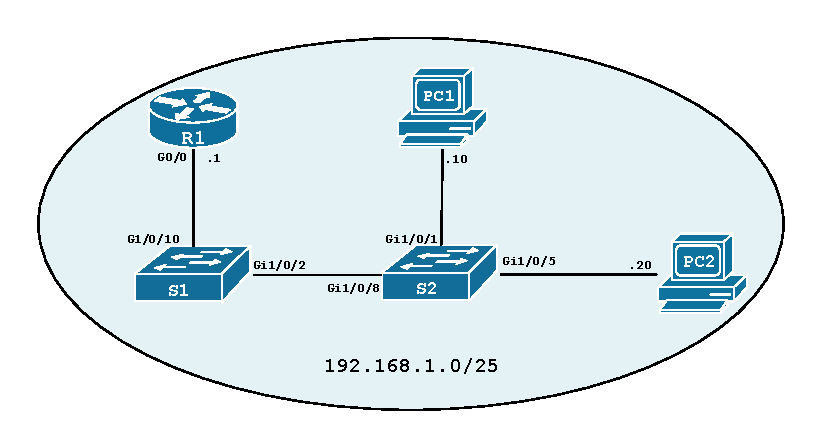
\includegraphics[width=0.7\linewidth]{topology-2}
	\caption{Η νέα μορφή της τοπολογίας.}\label{fig:topology-2}
\end{figure}

Έχοντας εφαρμόσει την κατάλληλη συνδεσμολογία που παραβιάζει τους κανόνες ασφαλείας, στείλτε πακέτα ICMP από τους υπολογιστές προς τον δρομολογητή. Πρέπει να επιτρέπεται στον PC2 να στέλνει πλαίσια προς τον R1, ενώ στον PC2 όχι. Παρατηρώντας το τερματικό κονσόλας του S1 καταγράψτε τα σχετικά μηνύματα syslog. 

\end{document}
